% !TeX program = pdflatex
\documentclass[border=6pt]{standalone}
\usepackage{tikz}
\usetikzlibrary{arrows.meta, positioning, chains}

\definecolor{MediumRed}{rgb}{0.925, 0.345, 0.345}
\definecolor{MediumGreen}{rgb}{0.37, 0.7, 0.66}
\definecolor{MediumBlue}{rgb}{0.015, 0.315, 0.45}
\definecolor{DarkBlue}{rgb}{0.05, 0.15, 0.35}

\begin{document}
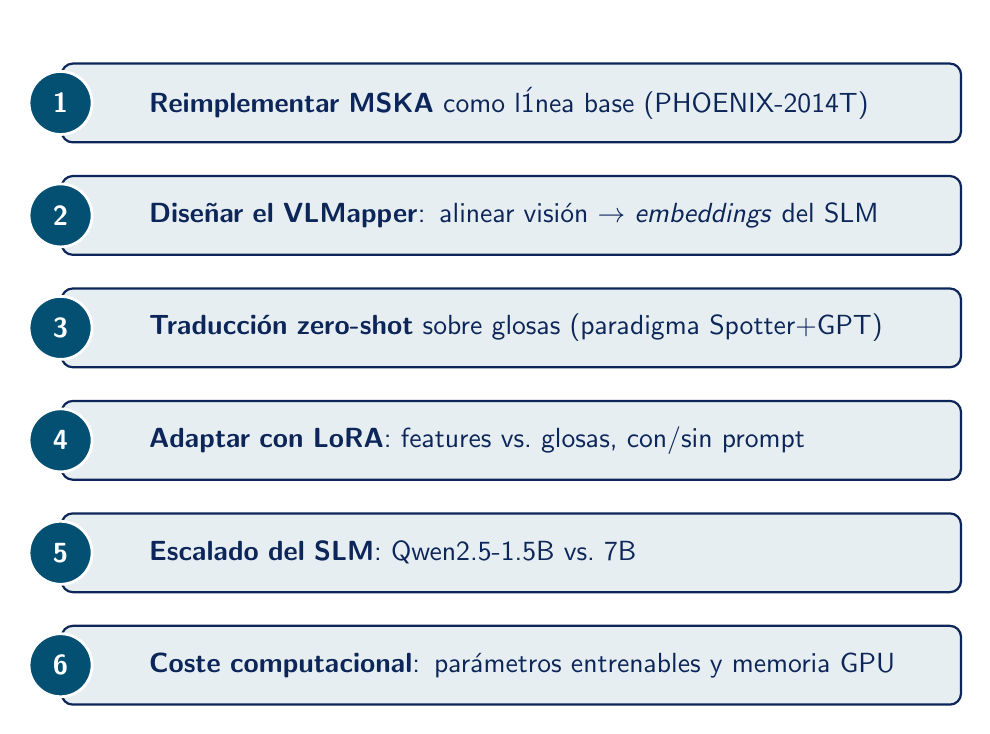
\begin{tikzpicture}[
    font=\sffamily,
    num/.style={circle, draw=white, line width=1pt, fill=MediumBlue,
        text=white, font=\sffamily\bfseries, minimum size=0.8cm, inner sep=0pt},
    paso/.style={draw=DarkBlue, thick, rounded corners=4pt, fill=MediumBlue!10,
        text=DarkBlue, align=left, text width=11cm, minimum height=1.0cm,
        inner sep=6pt},
    % Aumentamos el node distance para dar más aire entre filas
    node distance=4mm,
]

% Inicializamos un nodo invisible para poder posicionar el primer elemento
\node[inner sep=0pt] (s0) {};

\foreach \n/\txt [count=\i] in {%
    1/{\textbf{Reimplementar MSKA} como línea base (PHOENIX-2014T)},
    2/{\textbf{Diseñar el VLMapper}: alinear visión $\rightarrow$ \textit{embeddings} del SLM},
    3/{\textbf{Traducción \textit{zero-shot}} sobre glosas (paradigma Spotter+GPT)},
    4/{\textbf{Adaptar con LoRA}: features vs.\ glosas, con/sin prompt},
    5/{\textbf{Escalado del SLM}: Qwen2.5-1.5B vs.\ 7B},
    6/{\textbf{Coste computacional}: parámetros entrenables y memoria GPU}%
}{
    % Calculamos el índice anterior de forma segura en LaTeX
    \pgfmathtruncatemacro{\prev}{\i-1}

    % Posicionamos cada nodo exactamente debajo del anterior (s0, s1, s2...)
    \node[paso, below=of s\prev] (s\i) {\hspace{0.9cm}\txt};
    \node[num] at (s\i.west) {\n};
}

\end{tikzpicture}
\end{document}
